% !TEX root = tracking.tex
\section{Numerical examples} \label{sec:results}

In this section, we demonstrate the FaSTrack framework in three numerical examples involving a 5D car tracking a Dubins car model with the FSM planner, a 10D quadrotor tracking a single integrator model with the RRT planner, and an 8D quadrotor tracking a double integrator model with the MPC planner.
In each example, obstacles in the environment are \textit{a priori} unknown, and are revealed to the vehicle when they are sensed.
Whenever, obstacle map is updated, the planner re-plans a trajectory in real-time.
In this paper, the details of sensing are kept as simple as possible; we aim to only demonstrate our framework for real-time guaranteed safe planning and re-planning.
In general, any other planner can be used for planning in unknown environments, as long as planning and re-planning can be done in real-time.

For each example, we first describe the tracking and planning models. 
Next, we present the relative dynamics as well as the precomputation results. 
Afterwards, we briefly describe the planning algorithm and how obstacles are sensed by the vehicle. 
Finally, we show trajectory simulation results.

\subsection{5D car-3D car example with FSM \label{sec:reach_planner}}

For our first example, we demonstrate the combination of fast planning and provably robust tracking by combining fast sweeping method (FSM) \cite{Takei2013} with our computed TEB. 
FSM is an efficient optimal control-based planner for car-like systems, and provides numerically convergent globally optimal trajectory in real-time.

In this example, we use FSM to perform real-time planning for the 3D kinematic car model, whose trajectory is tracked by the 5D car model.
The dynamics of these models are given in \eqref{eq:5D_and_3D_dyn}.
The model parameters are chosen to be $a \in [-0.5, 0.5]$, $|\alpha|\le 6$, $\hat v = 0.1$, $|\hat\omega|\le 1.5$, $|\dstb_x|, |\dstb_y|, |\dstb_\alpha|\le0.02$, $|\dstb_a| \le 0.2$.

\subsubsection{Offline computation}

Using the relative system dynamics given in \eqref{eq:5D_and_3D_rdyn}, we defined the error function to be $\errfunc(\rstate) = x_\rstate^2 + y_\rstate^2$, and computed $\valfunc_\infty(\rstate)$, which is shown in Fig. \ref{fig:vf_TEB:5D3D}.
The minimum of the value function was approximately $\underline\valfunc = 0.004$, and the size of the TEB in $(x_r, y_r)$ space is approximately $0.065$.

The top left plot shows the TEB $\TEB_{\pstate, \infty}$, which is obtained from \eqref{eq:TEBp:inf}, in green.
The tracking model, which represents the system of interest, must apply the optimal control \eqref{eq:opt_ctrl} when it is on the green boundary.
The cross sectional area of the TEB is the largest area in when $\theta_r = 0, \pi$. 
This agrees with intuition, since at these $\theta_r$ values the 5D car model is either aligned with or opposite to the 3D car model.
Since the 5D car is able to move both forward and backward, these two alignments make tracking the easiest.
For the same reasoning, the cross sectional area is the smallest at $\theta_r = -\pi/2, \pi/2,$ etc.

The magenta and cyan planes indicate slices of the TEB at $\theta_r = \pi/2, -3\pi/4$, respectively.
With these $\theta_r$ values fixed, corresponding projections of the value function onto $(x_r, y_r)$ space are shown in the top right and bottom left plots.
Here, $\underline\valfunc$ is shown as the gray plane, with the intersection of the gray plane and the value function projection shown by the curve in the $0$-level plane. 
These curves are slices of $\TEB_{\pstate, \infty}$ at the $\theta_r = \pi/2, -3\pi/4$ levels.

Computation was done on a desktop computer with an Intel Core i7 5820K processor, on a $41\times41\times59\times35\times61$ grid, and took approximately 125 hours and required approximately 10 GB of RAM using a C++ implementation of level set methods for solving \eqref{eq:HJVI}.

\subsubsection{Online sensing and planning}
The simulation showing the combination of tracking and planning is shown in Fig. \ref{fig:5D3Dsim}.
The goal of the system, the 5D car, is to reach the blue circle at $(0.5, 0.5)$ with a heading that is within $\pi/6$ of the direction indicated by the arrow inside the blue circle, $\pi/2$.
Three initially unknown obstacles, whose boundaries are shown in dotted black, make up the constraints $\constr$.

While planning a trajectory to the goal, the car also senses obstacles in the vicinity.
For this example, we chose a simple virtual sensor that reveals obstacles within a range of $0.5$ units and in front of the vehicle within an angle of $\pi/6$.
This sensing region is depicted as the light green fan.

When a portion of the unknown obstacles is within this region, that portion is made known to the vehicle, and is shown in red.
These make up the sensed constraints $\constrSense$.
To ensure that the 5D car does not collide with the obstacles despite error in tracking, planning is done with respect to augmented constraints $\constrAug$, shown in dashed blue.

Given the current planning constraints $\constrAug$, the 3D planning system plans, in real-time using FSM, towards the goal.
This plan is shown in dotted black.
The 5D system robustly tracks the 3D system within the TEB in Fig. \ref{fig:vf_TEB:5D3D}.

Fig. \ref{fig:5D3Dsim} shows four time snapshots of the simulation.
In the top left subplot, the system has sensed only a very small portion of the obstacles, and hence plans a trajectory through an unknown obstacle to the target.
However, while tracking this initial trajectory, more of the L-shaped obstacle is made known to the system, and therefore the system plans around this obstacle, as shown in the top right subplot.
The bottom subplots show that eventually more obstacles are made known, and the system reaches the goal at $t=23.9$.

The simulation was done in MATLAB on a desktop computer with an Intel Core i7 2600K CPU.
Time was discretized in increments of $0.1$.
Averaged over the duration of the simulation, planning with FSM took approximately $0.066$ seconds per iteration, and obtaining the tracking controller from \eqref{eq:opt_ctrl} took approximately $0.0018$ seconds per iteration.

\begin{figure}
  \centering
  \begin{subfigure}[t]{0.49\columnwidth}
    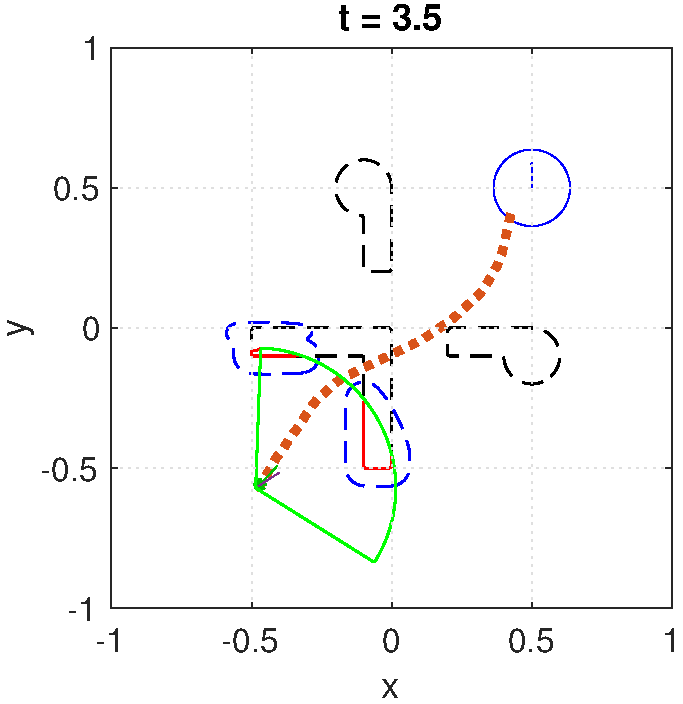
\includegraphics[width=\columnwidth]{fig/P5D_Dubins/36}
  \end{subfigure}
  \begin{subfigure}[t]{0.49\columnwidth}
    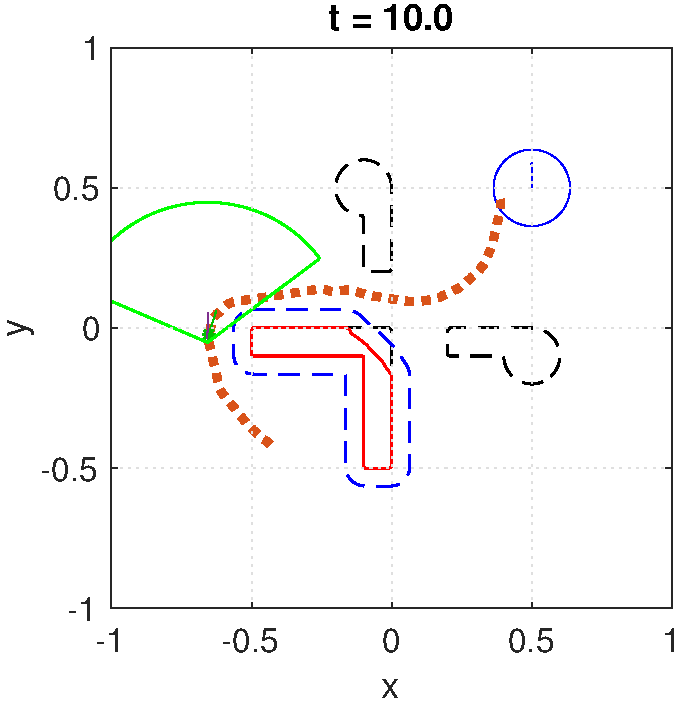
\includegraphics[width=\columnwidth]{fig/P5D_Dubins/101}
  \end{subfigure}  

  \begin{subfigure}[t]{0.49\columnwidth}
    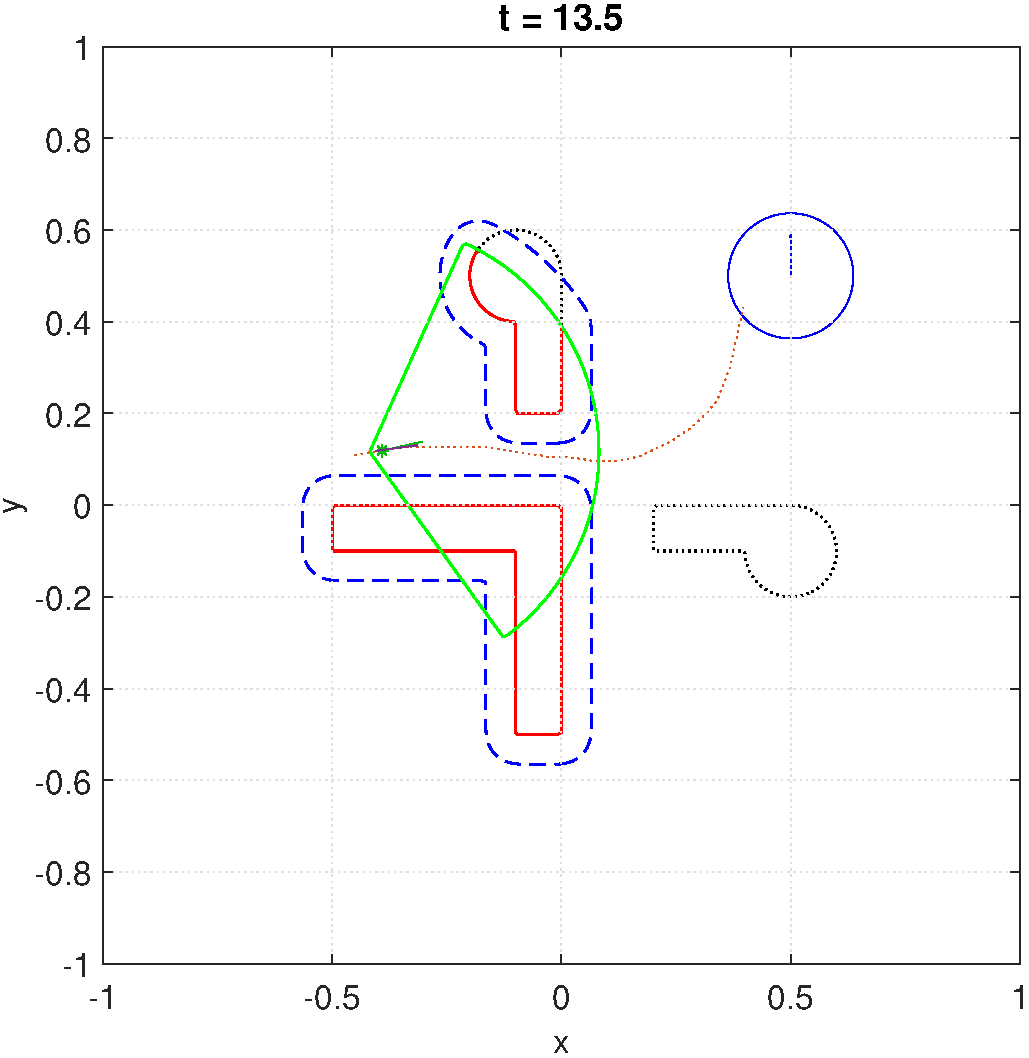
\includegraphics[width=\columnwidth]{fig/P5D_Dubins/136}
  \end{subfigure}
  \begin{subfigure}[t]{0.49\columnwidth}
    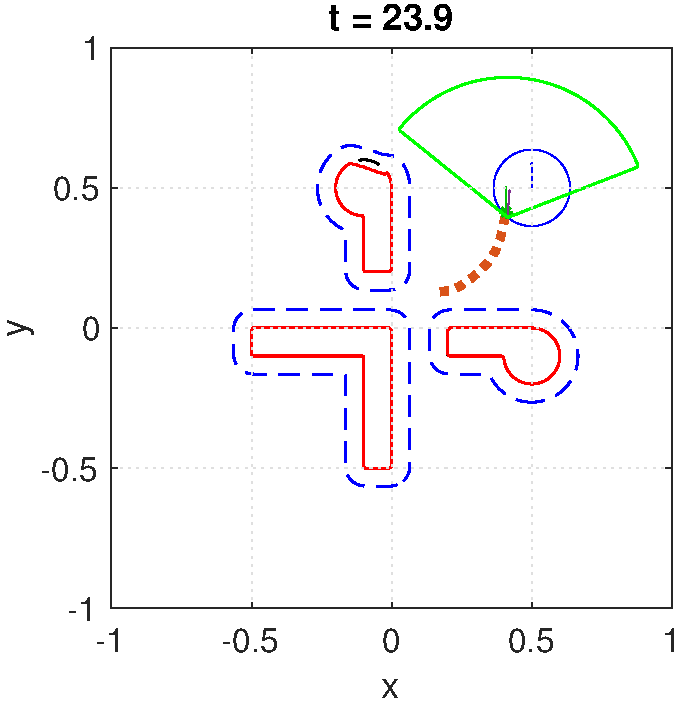
\includegraphics[width=\columnwidth]{fig/P5D_Dubins/240}
  \end{subfigure}
  \caption{Simulation of the 5D-3D example. As the vehicle with 5D car dynamics senses new obstacles in the sensing region (light green), the 3D model replans trajectories, which are robustly tracked by the 5D system. Augmentation of the constraints resulting from the obstacles ensures safety of the 5D system using the optimal tracking controller.} \label{fig:5D3Dsim}
\end{figure}